\documentclass[14pt,aspectratio=169,xcolor=dvipsnames]{beamer}
\usetheme{SimplePlus}
\usepackage{booktabs}
\usepackage{minted}

\title[short title]{Clase 3: Lenguajes de programación}
\subtitle{}
\author[NA Barnafi] {Nicolás Alejandro Barnafi Wittwer}
\institute[UC|CMM] 
{
    Pontificia Universidad Católica de Chile \\
    Centro de Modelamiento Matemático
}

\titlegraphic{
    \vspace{-1.8cm}
    \begin{flushright}
      
\includegraphics[height=2.5cm]{../images/logos/puc.png} 
    \end{flushright}
}

\date{14/08/2024}
\setbeamercovered{transparent}

\begin{document}
%%%%%%%%%%%%%%%%%%%%%%%%%%%%%%%%%%%%%%%%%%%%%%%%%%%%%%%
\begin{frame}
    \maketitle
\end{frame}
%%%%%%%%%%%%%%%%%%%%%%%%%%%%%%%%%%%%%%%%%%%%%%%%%%%%%%%
\section{Compilación de código}
%%%%%%%%%%%%%%%%%%%%%%%%%%%%%%%%%%%%%%%%%%%%%%%%%%%%%%%
\begin{frame}[t]\frametitle{La compilación}
    \idea{Consiste en traducir nuestro lenguaje al del PC}

    \vspace{1cm}
    \begin{itemize}
        \item<+-> Lo que nosotros entendemos: Lenguaje
        \item<+-> Lo que entiende el computador: 
    
        100010101010110101011010110101011011010101011101010000
            
    \end{itemize}
\end{frame}
%%%%%%%%%%%%%%%%%%%%%%%%%%%%%%%%%%%%%%%%%%%%%%%%%%%%%%%
\begin{frame}[fragile]\frametitle{Ejemplo de compilación}
\begin{small}
    \begin{columns}
        \begin{column}[b]{0.4\textwidth}
            \begin{minted}{C}
#include <stdio.h>
   int main() {
   printf("Hello, World!\n");
return 0;
            }
            \end{minted}

    \vfill
            Para humanos
        \end{column}
        \begin{column}[b]{0.45\textwidth}
        
            \begin{minted}{gas}
    .file	"hello.c"
    .text
    .section	.rodata
.LC0:
    .string	"Hello, World!"
    .text
    .globl	main
    .type	main, @function
main:
.LFB0:
            \end{minted}

    \vfill
            Resultado para PC
        \end{column}
    \end{columns}
\end{small}
\end{frame}
%%%%%%%%%%%%%%%%%%%%%%%%%%%%%%%%%%%%%%%%%%%%%%%%%%%%%%%
\begin{frame}\frametitle{El trabajo de compilación}
    \begin{enumerate}
        \item Procesar el archivo con código
        \item Generar símbolos de programas
        \item Juntar símbolos para generar programa
    \end{enumerate}

    \pause \begin{center}
        \begin{tabular}{c | c}
           Pros    &   Contras \\ \midrule
         \alertGreen{Eficiente} &   \alert{Inflexible}  \\
        \end{tabular}
    \end{center}

\pause Ejemplos de programas compilados: \texttt{ls, cd, }$\hdots$
\end{frame}
%%%%%%%%%%%%%%%%%%%%%%%%%%%%%%%%%%%%%%%%%%%%%%%%%%%%%%%
\begin{frame}\frametitle{Alternativa}
Lenguajes compilados son eficientes pero...
    \begin{itemize}
        \item Más complejos
        \item Requieren recompilar constantemente
    \end{itemize}

\vspace{1cm}
\pause Alternativa: \textbf{Lenguajes interpretados}

\pause
    \begin{itemize}
        \item Muchos subprogramas pre-compilados
        \item No se compila, se ejecuta secuencialmente (una línea a la vez)
        \item Permiten una consola interactiva
    \end{itemize}
\end{frame}
%%%%%%%%%%%%%%%%%%%%%%%%%%%%%%%%%%%%%%%%%%%%%%%%%%%%%%%
\begin{frame}\frametitle{Algunos ejemplos}
    \begin{columns}
        \begin{column}{0.45\textwidth}
            Compilados
            \begin{itemize}
                \item C/C++/C\#
                \item Java
                \item Rust
            \end{itemize}
        \end{column}

        \begin{column}{0.45\textwidth}
            Interpretados
            \begin{itemize}
                \item Python
                \item R
                \item MATLAB
                \item Julia
            \end{itemize}
        \end{column}
    \end{columns}
\end{frame}
%%%%%%%%%%%%%%%%%%%%%%%%%%%%%%%%%%%%%%%%%%%%%%%%%%%%%%%
\begin{frame}\frametitle{Ranking de lenguajes}
    \begin{center}
        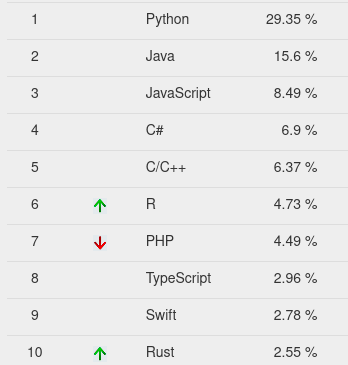
\includegraphics[width=0.4\textwidth]{../images/top-lenguajes.png}
    \end{center}
\end{frame}
%%%%%%%%%%%%%%%%%%%%%%%%%%%%%%%%%%%%%%%%%%%%%%%%%%%%%%%
\begin{frame}\frametitle{Más clasificaciones}
Los lenguajes también puede ser \emph{orientados a objetos}. Esto determina el nivel posible de abstracción.
    \begin{columns}
        \begin{column}{0.45\textwidth}
            Con objetos
            \begin{itemize}
                \item C++/C\#
                \item Java
                \item Rust
                \item Python
            \end{itemize}
        \end{column}

        \begin{column}{0.45\textwidth}
            Sin objetos
            \begin{itemize}
                \item C
                \item R
                \item MATLAB
                \item Julia
            \end{itemize}
        \end{column}
    \end{columns}
\end{frame}
%%%%%%%%%%%%%%%%%%%%%%%%%%%%%%%%%%%%%%%%%%%%%%%%%%%%%%%
\begin{frame}\frametitle{Recap}
    \begin{itemize}
        \item Concepto de compilación
        \item Hay lenguajes no compilados
        \item Hay más categorías de lenguajes
    \end{itemize}
\end{frame}
%%%%%%%%%%%%%%%%%%%%%%%%%%%%%%%%%%%%%%%%%%%%%%%%%%%%%%%
\begin{frame}
    \maketitle
\end{frame}
\end{document}
